% The results document: rebuilt by `make report` from the saved results. Text here is fixed; every number
% comes from the generated tables (../paper/tables), figures (../paper/figures) and facts (generated/).
\documentclass[10pt]{article}
\usepackage[a4paper,margin=2.2cm]{geometry}
\usepackage[T1]{fontenc}
\usepackage{lmodern}
\usepackage{booktabs}
\usepackage{graphicx}
\usepackage{array}
\usepackage{float}
\usepackage{caption}
\usepackage[hidelinks]{hyperref}
\graphicspath{{../paper/figures/}}
% keep every table where it is input (the generated tables carry no placement option)
\floatplacement{table}{H}
\renewenvironment{table*}{\begin{table}}{\end{table}}
\newcommand{\builtat}{2026-10-22 11:04}
\newcommand{\nanalyses}{28}
\newcommand{\nunits}{1}
\newcommand{\datasets}{NQ}
\newcommand{\seeds}{0}
\newcommand{\thesiscommit}{6039b30}
\newcommand{\model}{ollama\_llama3\_8b}


\title{Trust for multi-source RAG under attack:\\ results across datasets and seeds}
\author{Generated from the saved runs}
\date{Built \builtat}

\begin{document}
\maketitle

\noindent\textbf{Scope.} \nanalyses{} analyses over \nunits{} dataset--seed runs (datasets: \datasets; seeds: \seeds).
Every method answers the same cached LLM answers (\model{}, thesis code at \thesiscommit), so differences come only
from how sources are trusted and how the answer is chosen. Each setup has 9 sources (5 for the honest mix, 7 for the
domain experts) with 200 warm-up and 600 test questions; RA-RAG's answering asks $\kappa = 4$ sources; accuracy uses
the fair match.

\section{Summary of results}
Each result of the first evaluation series is a comparison between a baseline and a method on the same test
questions. Table~\ref{tab:claims} gives the difference on every dataset and over all runs, Figure~\ref{fig:claims}
the same with its interval.

\begin{table*}
\centering
\small
\begin{tabular}{@{}l p{6.2cm} rrr r c@{}}
\toprule
\# & Result (method vs baseline) & NQ & TriviaQA & HotpotQA & All, 95\% CI & Holds \\
\midrule
1 & RA-RAG beats equal weights (the paper's result): RA-RAG (paper) vs equal weights, accuracy & $+3.3$ & -- & -- & $+3.3$ & 1/1 \\
2 & RA-RAG's estimate overrates some sources: RA-RAG's estimate, largest excess vs warm-up truth, estimate minus truth (score) & -- & -- & -- & -- & -- \\
3 & Frozen trust is easy to attack (2 attackers of 9): SL with aging vs RA-RAG frozen (paper), attacks that succeed & $-40.1$ & -- & -- & $-40.1$ & 1/1 \\
4 & Staying online recovers most of it (3 attackers): RA-RAG online vs RA-RAG frozen, accuracy & $+21.0$ & -- & -- & $+21.0$ & 1/1 \\
5a & Forgetting is the defense: SL (late switch): SL with aging vs SL online, accuracy & -- & -- & -- & -- & -- \\
5b & Forgetting is the defense: RA-RAG (late switch): RA-RAG with a window vs RA-RAG online, accuracy & -- & -- & -- & -- & -- \\
6 & Same memory: SL and RA-RAG tie (1-3 attackers): SL with a window vs RA-RAG with a window, accuracy & $+0.4$ & -- & -- & $+0.4$ [$+0.1$, $+0.6$] & 3/3 \\
7 & The switch detector adds little: SL with aging + the detector vs SL with aging, accuracy & $-0.2$ & -- & -- & $-0.2$ & 1/1 \\
8 & SL is better with few warm-up questions (5 sources, 5 questions): SL frozen vs RA-RAG frozen, accuracy & -- & -- & -- & -- & -- \\
9a & SL holds better near a majority of attackers (4 of 9): SL with a window vs RA-RAG with a window, accuracy & $+7.0$ & -- & -- & $+7.0$ & 1/1 \\
9b & ... and fewer attacks succeed: SL with a window vs RA-RAG with a window, attacks that succeed & $-13.6$ & -- & -- & $-13.6$ & 1/1 \\
10 & Learning a trust is essential (7 unreliable of 9): best learned trust vs equal weights, accuracy & $+38.8$ & -- & -- & $+38.8$ & 1/1 \\
11 & One score per source rarely asks the experts: RA-RAG (paper) vs equal weights, accuracy & -- & -- & -- & -- & -- \\
12a & Trust per domain, online (SL, 15 warm-up questions): SL per domain vs SL, one score, accuracy & -- & -- & -- & -- & -- \\
12b & Trust per domain, frozen (SL, 15 warm-up questions): SL frozen per domain vs SL frozen, one score, accuracy & -- & -- & -- & -- & -- \\
13a & Without labels, soft weights recover part of the gain: SL, soft weights vs SL, no domains, accuracy & -- & -- & -- & -- & -- \\
13b & Soft weights beat the nearest centroid: SL, soft weights vs SL, nearest centroid, accuracy & -- & -- & -- & -- & -- \\
14a & SL beats RA-RAG per domain (LLM labels): SL per domain vs RA-RAG per domain, online, accuracy & -- & -- & -- & -- & -- \\
14b & SL beats RA-RAG per domain (nearest centroid): SL per domain vs RA-RAG per domain, online, accuracy & -- & -- & -- & -- & -- \\
15 & SL's own answering protects out-of-date trust (frozen, 3 attackers): SL's own answering vs RA-RAG's answering, attacks that succeed & $-26.8$ & -- & -- & $-26.8$ & 1/1 \\
\bottomrule
\end{tabular}
\caption{The first evaluation series' results across datasets and seeds. Each cell is the method's difference from the baseline in percentage points (accuracy or attacks that succeed), averaged over seeds; ``All'' averages every dataset and seed, with a 95\% $t$ interval when there are several; ``Holds'' counts the runs where the difference goes the expected way (for a tie: within one point).}
\label{tab:claims}
\end{table*}


\begin{figure}[H]
\centering
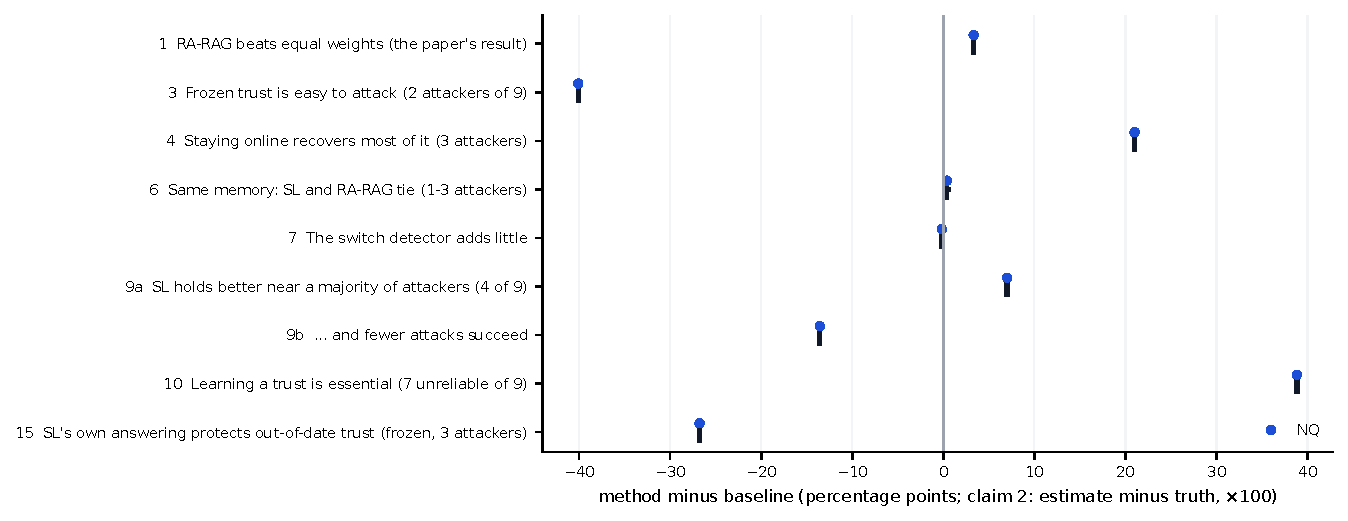
\includegraphics[width=\linewidth]{claims_forest}
\caption{Method minus baseline for each result (percentage points): per dataset (markers) and over every dataset and
seed (bar: mean; line: 95\% interval).}
\label{fig:claims}
\end{figure}

\section{Attacks and forgetting}
Coordinated attackers answer honestly through the warm-up, then all give the same wrong answer on half the test
questions. A trust frozen after the warm-up keeps trusting them; a trust that keeps learning and forgets old evidence
does not. Tables~\ref{tab:attackers_accuracy} and~\ref{tab:attackers_attack}, Figure~\ref{fig:attackers}.

\begin{table}
\centering
\small
\begin{tabular}{@{}lrrrr@{}}
\toprule
Trust & 1 of 9 & 2 of 9 & 3 of 9 & 4 of 9 \\
\midrule
\multicolumn{5}{@{}l}{\textit{NQ}} \\
\quad RA-RAG, frozen (paper) & 84.7 & 68.2 & 58.5 & 52.0 \\
\quad RA-RAG online & 86.0 & 82.7 & 79.5 & 51.3 \\
\quad RA-RAG, window of 100 & 86.3 & 85.8 & 83.5 & 56.2 \\
\quad SL, frozen & 86.0 & 69.3 & 59.2 & 53.0 \\
\quad SL online, no forgetting & 86.0 & 83.7 & 78.0 & 53.2 \\
\quad SL, aging $\lambda=0.97$ & 86.8 & 86.0 & 83.5 & 63.3 \\
\quad SL, window of 100 & 86.8 & 86.2 & 83.8 & 63.2 \\
\quad Equal weights & 85.8 & 80.5 & 75.7 & 56.8 \\
\bottomrule
\end{tabular}
\caption{Coordinated build-then-betray attackers among 9 sources (and 3 attackers switching halfway through the test): accuracy in percent, mean over seeds with the spread as a subscript.}
\label{tab:attackers_accuracy}
\end{table}

\begin{table}
\centering
\small
\begin{tabular}{@{}lrrrr@{}}
\toprule
Trust & 1 of 9 & 2 of 9 & 3 of 9 & 4 of 9 \\
\midrule
\multicolumn{5}{@{}l}{\textit{NQ}} \\
\quad RA-RAG, frozen (paper) & 8.4 & 43.3 & 59.5 & 70.8 \\
\quad RA-RAG online & 0.6 & 6.9 & 14.1 & 72.5 \\
\quad RA-RAG, window of 100 & 0.6 & 1.6 & 6.7 & 63.1 \\
\quad SL, frozen & 1.7 & 42.1 & 58.8 & 69.5 \\
\quad SL online, no forgetting & 0.6 & 4.9 & 18.7 & 69.2 \\
\quad SL, aging $\lambda=0.97$ & 0.6 & 3.2 & 7.7 & 46.1 \\
\quad SL, window of 100 & 0.6 & 2.4 & 7.0 & 49.5 \\
\quad Equal weights & 1.1 & 11.7 & 21.5 & 61.7 \\
\bottomrule
\end{tabular}
\caption{The same setups: share of attacked questions answered with the attackers' answer, in percent.}
\label{tab:attackers_attack}
\end{table}


\begin{figure}[H]
\centering
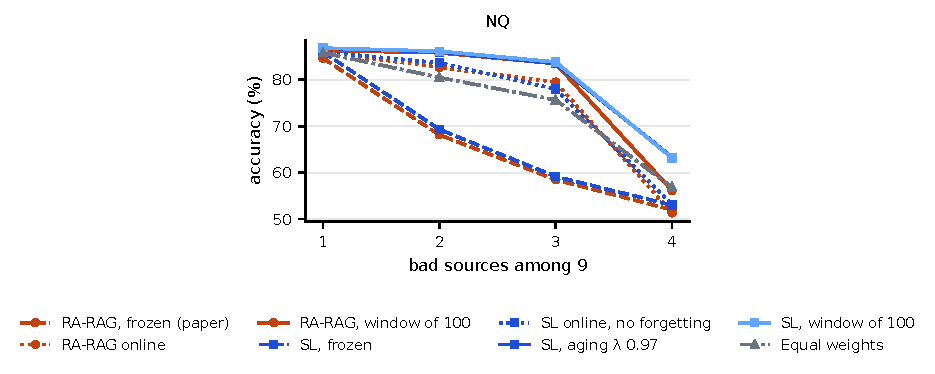
\includegraphics[width=\linewidth]{attackers_accuracy}\\[4pt]
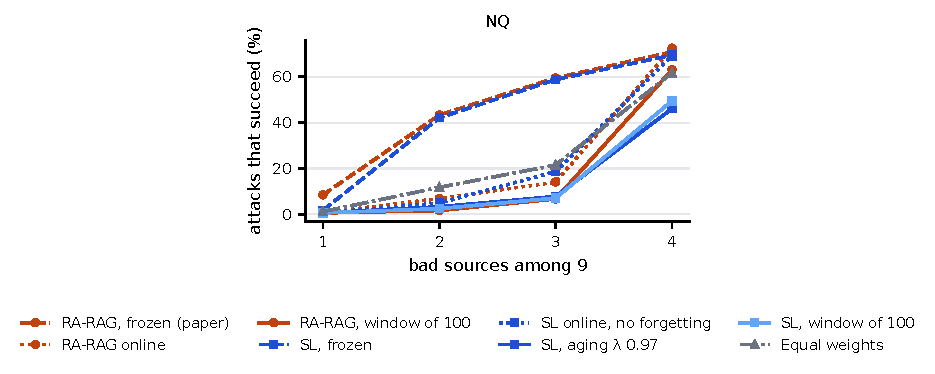
\includegraphics[width=\linewidth]{attackers_attack}
\caption{Accuracy (top) and attacks that succeed (bottom) against the number of attackers among 9 sources; mean over
seeds, band: range over seeds.}
\label{fig:attackers}
\end{figure}

\section{Unreliable sources}
Unreliable sources are right only 10\% of the time and disagree with each other. Learning any trust removes most of
their harm; equal weights does not (Table~\ref{tab:unreliable}).

\begin{table}
\centering
\small
\begin{tabular}{@{}lrr@{}}
\toprule
Trust & 3 of 9 & 7 of 9 \\
\midrule
\multicolumn{3}{@{}l}{\textit{NQ}} \\
\quad RA-RAG, frozen (paper) & 85.0 & 69.2 \\
\quad RA-RAG online & 85.5 & 69.5 \\
\quad RA-RAG, window of 100 & 85.8 & 69.7 \\
\quad SL, frozen & 84.8 & 71.3 \\
\quad SL online, no forgetting & 84.5 & 69.3 \\
\quad SL, aging $\lambda=0.97$ & 85.8 & 69.0 \\
\quad SL, window of 100 & 85.7 & 70.0 \\
\quad Equal weights & 81.7 & 32.5 \\
\bottomrule
\end{tabular}
\caption{Static unreliable sources (right 10\% of the time) among 9: accuracy in percent.}
\label{tab:unreliable}
\end{table}


\section{Few warm-up questions}
With a handful of warm-up answers, RA-RAG's estimate (a raw share of agreements) swings to extremes; SL's trust starts
from a prior and moves with the evidence (Table~\ref{tab:warmup}, Figure~\ref{fig:warmup}).

\begin{table}
\centering
\small
\begin{tabular}{@{}lrrr@{}}
\toprule
Dataset & 5 & 10 & 20 \\
\midrule
NQ & -- & -- & -- \\
TriviaQA & -- & -- & -- \\
HotpotQA & -- & -- & -- \\
\bottomrule
\end{tabular}
\caption{Few warm-up questions (five honest sources, reliabilities 0.53--0.91): SL's frozen trust minus RA-RAG's frozen estimate, accuracy in points, by number of warm-up questions; mean over random warm-up draws and seeds.}
\label{tab:warmup}
\end{table}


\begin{figure}[H]
\centering

\includegraphics[width=0.55\linewidth]{warmup}
\caption{SL's frozen trust minus RA-RAG's frozen estimate (accuracy points) by number of warm-up questions.}
\label{fig:warmup}
\end{figure}

\section{Domain experts}
Each expert is right 90\% of the time in its own domain and 30\% elsewhere; two generalists are right 60\% of the
time everywhere. The system is never told who is an expert. Trust is learned per domain, with each question placed
among the domains by the LLM's label, by the nearest domain centroid of its embedding, or by soft weights over the
domains (Table~\ref{tab:domains}, Figure~\ref{fig:domains}).

\begin{table}
\centering
\small
\begin{tabular}{@{}lrr@{}}
\toprule
Domain of a question & \multicolumn{2}{c}{NQ} \\
 & SL & RA-RAG \\
\midrule
No domains & -- & -- \\
LLM's labels & -- & -- \\
Nearest centroid & -- & -- \\
Soft weights & -- & -- \\
\bottomrule
\end{tabular}
\caption{Domain experts (right 90\% of the time in their domain, 30\% elsewhere): accuracy with trust learned per domain online, by how each question is placed among the domains, full warm-up. RA-RAG's estimator runs per domain on each question's top domain.}
\label{tab:domains}
\end{table}


\begin{figure}[H]
\centering

\includegraphics[width=0.55\linewidth]{domains}
\caption{SL's accuracy with trust per domain, by how questions are placed among domains (mean over seeds, bar: range).}
\label{fig:domains}
\end{figure}

\section{SL's own answering}
Instead of RA-RAG's vote over the four most trusted sources, SL can answer by itself: it asks every source, fuses
their evidence, and answers, says \emph{unknown}, or says \emph{conflict} and shows two answers (Table~\ref{tab:answering}).

\begin{table*}
\centering
\small
\begin{tabular}{@{}lrrrrrrr@{}}
\toprule
Setup & Answers & Right & RA-RAG, same cov. & Conflict right & Unknown wrong & \multicolumn{2}{c}{Attacks succeed} \\
 & & & & & & SL & RA-RAG \\
\midrule
3 unreliable of 9 & 70.8 & 90.6 & 89.6 & 63.2 & 35.8 & -- & -- \\
7 unreliable of 9 & 0.0 & -- & -- & -- & 50.8 & -- & -- \\
1 attacker of 9 & 90.2 & 89.5 & 89.5 & 64.3 & 55.9 & 0.0 & 0.6 \\
2 attackers of 9 & 89.2 & 88.4 & 88.4 & 73.7 & 50.0 & 2.0 & 3.2 \\
3 attackers of 9 & 83.5 & 85.2 & 87.6 & 87.0 & 55.6 & 10.2 & 7.7 \\
4 attackers of 9 & 79.7 & 69.5 & 69.0 & 84.2 & 54.3 & 38.0 & 46.1 \\
\bottomrule
\end{tabular}
\caption{SL's own answering (answer, \emph{unknown} or \emph{conflict}) with its online trust and aging: share of questions answered, accuracy on those, RA-RAG's accuracy on its most confident questions at the same coverage and trust, conflicts whose two answers include the right one, \emph{unknown} questions whose top answer would have been wrong, and attacks that succeed with SL's answering and with RA-RAG's on the same trust. Means over all datasets and seeds.}
\label{tab:answering}
\end{table*}


\appendix
\section{Runs}
\begin{table}
\centering
\small
\begin{tabular}{@{}lc@{}}
\toprule
Dataset & seed 0 \\
\midrule
NQ & 28/28 \\
\bottomrule
\end{tabular}
\caption{Analyses saved per dataset and seed, out of those planned.}
\label{tab:status}
\end{table}


\end{document}
